\documentclass{sig-alternate}
	\usepackage{algorithm}
	\usepackage{algpseudocode}
	\usepackage{listings}
	\usepackage{subfigure}

	\usepackage{tikz}
	\usepackage{tikz-uml}
	\tikzumlset{draw=black}
	\tikzumlset{fill class=white}
	\tikzumlset{fill template=white}
	\tikzumlset{fill package=white}

	\usepackage{pgf-umlsd}
	\usepgflibrary{arrows} % for pgf-umlsd

	\usepackage{bytefield}

	\usepackage{fourier}
	\usepackage{enumitem}

	\newcommand{\invitro}{\emph{in vitro} }
\begin{document}

\title{High-Level Sprout Geometry Extraction for In Vitro Angiogenesis Assays}
\numberofauthors{4}
\author{
	\alignauthor Gio Borje \\
		\affaddr{University of California, Irvine} \\
		\email{gborje@uci.edu}
	\alignauthor Craig Steinke \\
		\affaddr{University of California, Irvine} \\
		\email{steinkec@uci.edu}
}
\date{\today}
\maketitle

\begin{abstract}
	We have developed an automated system for the quantitative analysis of
	\invitro angiogenesis assays. Specifically, the system is designed to
	analyze fibrin gel bead sprouting assays developed by the laboratory
	of Dr. Chris Hughes in the Department of Molecular Biology \&
	Biochemistry at UC Irvine. Our system enumerates sprouts for each
	bead and calculates the average branching factor and the average
	length for an imaged assay. Our approach reports accurate sprout
	enumeration when compared with manual counts by an expert observer
	while significantly reducing the analysis time.
\end{abstract}

\section{Introduction} % (fold)
\label{sec:Introduction}
	%% Motivation
	Angiogenesis is a mechanism for the formation of new blood vessels
	from pre-existing vessels. Tumor angiogenesis in solid tumors is
	thought to facilitate the transition from a benign tumor to a
	malignant phenotype. Additionally, the avascular growth phase allows
	for an an approximate maximum size of 1--2mm in diameter; on the other
	hand, the vascular growth phase enables unyielding tumor expansion
	and metastasis \cite{kerbel99}. Subsequently, the analysis of
	\invitro angiogenesis assays is necessary to assess the impact of
	pro-angiogenic and anti-angiogenic agents.

	%% Acknowledge existing methods
	Niemisto et. al developed a general image analysis method for the
	quantification of similar \invitro angiogenesis assays. Their method
	provides the length and size of each tubule complex as well as the number
	of junctions within them \cite{niemisto05}. The TCS Cellworks Angiokit
	(Buckingham, UK) images used by Niemisto et. al have two distinguishable
	and ideal properties in contrast to our images that require us to use a
	variant approach. First, their images have tubule complexes that are
	solidly filled whereas our images have visible lumens. Second, their images
	show no distinguishable origin for sprouts whereas our images have a bead
	from which sprouts originate. Hence, we propose a modified methodology for
	our image set.

	%% Reference the Hughes Lab FBGSA
	The image set under analysis is provided by the Hughes Lab. Their
	fibrin bead assay using human umbilical vein endothelial cells (HUVEC)
	contrasts with fibrin bead assays containing Bovine aortic endothelial
	cells (BAEC). HUVEC have been the canonical EC model system and more
	accurately represents angiogenesis in humans. The assay begins by
	culturing HUVEC as a monolayer on dextran-coated Cytodex beads. This
	method induces HUVEC to recapitulate multicellular capillaries in
	fibrin gels.  Furthermore, the method for HUVEC promotes sprouting,
	lumen formation and long-term stability of neovessels. The
	high-resolution images of beads are then captured on an IX70 Olympus
	microscope \cite{nakatsu03}. A sample image can be seen on Figure
	\ref{fig:monobead}.

	\begin{figure}[ht]
		\centering
		\includegraphics[width=6cm]{images/mono.jpg}
		\caption{Single Bead Image from the Hughes Lab Images}
		\label{fig:monobead}
	\end{figure}

	%% How sprout counts were previously acquired
	Previously, the number of sprout counts per bead were measured by manual
	counting on the obtained images. Furthermore, the sprout length was
	ambiguously measured in arbitrary units \cite{nakatsu03}. Our system
	relieves the laborious, manual analysis by quickly automating the detection
	and reliably analyzing of imaged assay features.

	%% Overview of the system
	Our system, the High-Level Sprout Geometry (HLSG) Extractor, is designed to
	detect features, restore features and analyze the features of imaged
	assays. Features for detection include the Cytodex bead and its associated
	multicellular capillaries. Due to the noise and depth of the image, the
	HLSG Extractor uses structural inpainting to infer which sprout segments
	emerge belong the same sprout. After structural inpainting, the HLSG
	Extractor quantitatively analyzed the images using Sholl Analysis to
	determine the number of primary sprouts, the average length and the average
	branching factor for each bead in the imaged assay.

	In addition to the High-Level Sprout Geometry (HLSG) Extractor, a driver
	and report generator are implemented to drive functionality on sample
	images and generate reports on the analyses respectively.

	The following sections will proceed as follows. Section
	\ref{sec:Methodology} will describe an overview of the HLSG feature
	detection, feature restoration and analysis mechanisms. Section
	\ref{sec:Data Structures} will describe the data structures used to
	represent the HLSG and its properties. Section \ref{sec:System
	Architecture} shows how the system is designed for modularity and
	robustness.
% section Introduction (end)

\section{Methodology} % (fold)

%% SHOLL ANALYSIS
%% Statistical Analysis

%% BEAD DETECTION
%% Edge Detection
%% Hough Transform

%% NON-BEAD DETECTION
%% Bead Masking
%% Edge Detection
%% Thickening
%% Thinning
%% Pruning

\label{sec:Methodology}
	Our system enables feature set detection, minor feature restoration and
	quantitative analysis which can be decomposed into four stages. The
	first two stages detect feature sets: beads as features and then
	sprouts as features. In the third stage, the system attempts to restore
	a few sprout features by approximating and inpainting connections between
	broken sprout segments as well as filling holes. Finally, the system
	quantitatively analyzes the imaged assays through Sholl Analysis.

	\begin{figure}[htp!]
		\centering
		\subfigure[Sprout Segments]{
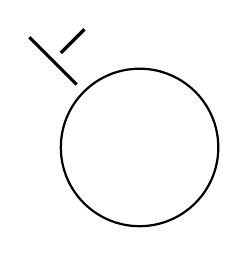
\begin{tikzpicture}
	\node [draw, thick, circle, text centered,  minimum size=2cm] at (0,0) {}; 
	%% BL Sprout
	\draw [very thick] (-0.8,0.8) -- +(-0.6,0.6);
	\draw [very thick] (-1,1.2) -- +(0.3,0.3);
	%\node at (-1.2, -2) {$(d)$};
\end{tikzpicture}
}
\subfigure[Branching]{
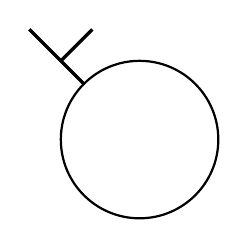
\begin{tikzpicture}
	\node [draw, thick, circle, text centered,  minimum size=2cm] at (0,0) {}; 
	%% TL Sprout
	\draw [very thick] (-0.7,0.7) -- +(-0.7,0.7);
	\draw [very thick] (-1,1) -- +(0.4,0.4);
	%\node at (-1, 2) {$(c)$};
\end{tikzpicture}
}
\subfigure[Junction Point]{
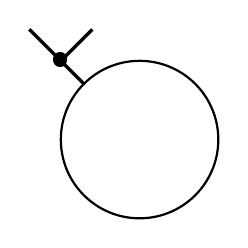
\begin{tikzpicture}
	\node [draw, thick, circle, text centered,  minimum size=2cm] at (0,0) {}; 
	%% TL Sprout
	\draw [very thick] (-0.7,0.7) -- +(-0.7,0.7);
	\draw [very thick] (-1,1) -- +(0.4,0.4);
	\node at (-1,1) {\Large\textbullet};
	%\node at (-1, 2) {$(c)$};
\end{tikzpicture}
}

		\caption{Branching Geometry}
		\label{fig:beadex}
	\end{figure}

	\subsection{Bead Extraction} % (fold)
	\label{sub:Bead Extraction}
		\begin{figure}[htp!]
			\centering
			% \subfigure[Original]{\includegraphics[width=4.1cm]{images/mono.jpg}}
			\subfigure[Edges]{\includegraphics[width=4.1cm]{images/mono_preprocessed.jpg}}
			\subfigure[Bead Detection]{\includegraphics[width=4.1cm]{images/mono_found_circle.jpg}}
			\caption{Bead Extraction Outline}
			\label{fig:beadex}
		\end{figure}
		Bead extraction is a two-step process. To reduce noise, the system
		first smooths the image using a Gaussian blur. Second, circles in
		the image are detected using the circular Hough Transform. The
		circles detected correspond to the beads in the assay. It follows that
		the origin and radius of the bead is obtained.

		In order to avoid false bead detections, we enforce that the minimum
		distance between the origin of every pair of detected circles be four
		times the average bead radius i.e. each detected bead should at least
		be a bead apart. Beware that we ignore the degenerate case in which two
		or more beads are within the distance constraint because associating
		sprouts to beads becomes inaccurate.
	% subsection Bead Extraction (end)

	\subsection{Sprout Extraction} % (fold)
	\label{sub:Sprout Extraction}
		\begin{figure}[htp!]
			\centering
			\subfigure[Dilated]{\includegraphics[width=4.1cm]{images/mono_dilated.jpg}}
			\subfigure[Skeleton]{\includegraphics[width=4.1cm]{images/mono_skeletonized.jpg}}
			\caption{Sprout Extraction Outline}
			\label{fig:beadex}
		\end{figure}

		Sprout extraction depends on bead extraction because the beads must be
		masked before sprout extraction occurs to separate beads from sprouts.
		We mask the beads given the geometry of the circles. Due to the
		disconnectivity of sprouts in the assay, we begin by obtaining all
		sprout segments and represent them as line segments. We distinguish the
		end points of each line segment for connectivity. The start point, $S$,
		is the end point on the line segment such that it is closer to the
		origin of the line segment's closest bead. The end point, $E$, is the
		end point on the line segment such that it is farther from the origin
		of the line segment's closest bead.

		To determine which line segments belong to the same sprout, we use
		Euclidean distance between their start and end points enforced by
		the constraint that the end point must be closer to the origin of
		its closest bead than the target start point. For example, two
		line segments are part of the same sprout if the distance between
		the start an end points are within a specified distance parameter,
		$d$.
	% subsection Sprout Extraction (end)

	\subsection{Sprout Restoration} % (fold)
	\label{sub:Sprout Restoration}
		There are two primary sources of degradation that we have discovered in
		the imaged assays: disjoint sprout segments and false capillary lumen
		detections i.e. holes. We will discuss our approaches to both problems
		independently. 
		
		The disjoint sprout segments are caused by the three-dimensional nature
		of the sprouts moving in and out of focus of the microscope.
		
		False capillary lumen detections are artifacts of the Canny
		edge-detection algorithm. By the morphology of these structures, we
		simply find the contours which enclose small holes and perform
		inpainting by polygon approximation using the Ramer-Douglas-Peucker
		algorithm.
	% subsection Sprout Restoration (end)

	\subsection{Sholl Analysis} % (fold)
	\label{sub:Sholl Analysis}
		Sholl Analysis is a quantitative method for quantitatively analyzing
		morphological characteristics of neurons \cite{sholl53}. Briefly, Sholl
		Analysis consists of counting the number of foreground to background
		crossings given concentric circles of a parameterized radius.

		\begin{algorithm}[ht!]
			\caption{Sholl Analysis}
			\begin{algorithmic}
				\Procedure{ShollAnalysis}{img, origin, radius}
					\State $r_{\min} \gets$ radius
					\State $r_{\max} \gets$ $\min\left\{\text{origin.x, img.width - origin.x}\right\}$
					\State $r_{\max} \gets$ $\min\left\{r_{\max}, \text{ origin.y, img.height - origin.y}\right\}$
					\State crossings $\gets$ empty dictionary
					\ForAll{$r \in [r_{\min}, r_{\max}]$}
						\State crossings[$r$] $\gets$ \Call{CountCrossings}{img, origin, $r$}
					\EndFor
					\State \Return crossings
				\EndProcedure
			\end{algorithmic}
			\begin{algorithmic}
				\Procedure{CountCrossings}{img, origin, radius}
					\State crossings $\gets$ 0
					\ForAll{pixel $\in$ \Call{BresenhamCircle}{origin, radius}}
						\If{crossing detected at pixel}
							\State crossings $\gets$ crossings + 1
						\EndIf
					\EndFor
					\State \Return crossings
				\EndProcedure
			\end{algorithmic}
		\end{algorithm}

	% subsection Sholl Analysis (end)
% section Methodology (end)

\section{Data Structures} % (fold)
\label{sec:Data Structures}
	The following data structures are used to implement the HLSG Extractor.
	\begin{figure}[!ht]
		\centering
		\begin{tikzpicture}
\umlclass[x=0,y=0]{BeadFeature}{
	+ center : (uint, uint) \\
	+ radius : uint \\
	}{}
\umlclass[x=4.5,y=0]{SproutFeature}{
	+ centroid : (uint, uint) \\
	+ length : uint \\
	+ width : uint \\
	}{}
\umlclass[x=4.5,y=-3]{RadialSegment}{
	+ inner : (uint, uint) \\
	+ outer : (uint, uint) \\
	+ blob : Blob
	}{}
%% Relations
\umlaggreg{BeadFeature}{SproutFeature}
\umluniaggreg{SproutFeature}{RadialSegment}
\end{tikzpicture}

		\caption{HLSG Extractor Features Class Diagram}
		\label{fig:classdiag}
	\end{figure}

	\subsection{Bead Feature} % (fold)
	\label{sub:Bead Feature}
		A bead feature is an abstraction of the Cytodex bead coated with
		endothelial cells in the assay. The geometry of the bead is intuitively
		circular; subsequently the geometry can is described by the descriptor
		in Figure \ref{fig:classdiag}.
	% subsection Bead Feature (end)

	\subsection{Sprout Feature} % (fold)
	\label{sub:Sprout Feature}
		A sprout feature is an abstraction of the blood vessels that develop
		through angiogenesis from the designed bead. Subsequently, sprout
		feature extraction is dependent upon bead descriptors. The sprout is
		actually comprised of a set of pixel segments because of the
		possibility that a sprout is disconnected.
	% subsection Sprout Feature (end)

	\subsection{Radial Line Segment} % (fold)
	\label{sub:Radial Line Segment}
		Due to the disconnectivity of sprouts, individual sprout segments
		are represented by a radially defined line segment. That is, we
		distinguish the end points from its radial distance from the origin
		of its corresponding bead. Given a line segment, we say that and
		end point is the \emph{inner point} if it is radially closer than
		its complementary end point; otherwise, we call the end point the
		\emph{outer point}.

		In addition to the distinguishable end points, a radial line
		segment is a line fit onto a corresponding blob of pixels which can
		be considered a sprout segment.
	% subsection Radial Line Segment (end)

	\subsection{Driver} % (fold)
	\label{sub:Driver}
		The Driver is responsible for parsing input from the user and emulating
		the encoded actions as functions of the HLSG Extractor. That is, the
		Driver acts similar to a REPL (Read-Eval-Print-Loop) that reads input
		from the user, evaluates the input and prints the corresponding output
		in a loop. The set of commands available to the user is outlined Table
		\ref{tab:commands}.
	% subsection Driver (end)
% section Data Structures (end)

\section{System Architecture} % (fold)
\label{sec:System Architecture}
	The system requires Python version 2.7x with the SimpleCV package. The
	architecture of the system is based on our methodology for
	quantitatively analyzing \invitro angiogenesis. The system, however,
	incorporates modules for driving batch processes as well as a
	Read-Eval-Print-Loop (REPL) for console interaction. Finally, a module
	incorporated for generating CSV reports of the analysis. The sequence
	diagram for the system components are shown in Figure
	\ref{fig:sysarch}.
	\begin{figure*}[ht!]
		\centering
		\centering
\begin{sequencediagram}
\newthread{client}{Client}{}
\newinst[1]{driver}{Driver}{}
\newinst[1]{hlsgex}{HLSG Extractor}{}
\newinst[1]{beadex}{Bead Extractor}{}
\newinst[1]{sproutex}{Sprout Extractor}{}
\newinst[1]{reportgen}{Report Generator}{}

\begin{call}{client}{images}{driver}{}
	\begin{sdblock}{Main Loop}{}
		\begin{call}{driver}{extract(img)}{hlsgex}{hlsg}
			\begin{call}{hlsgex}{extract(img)}{beadex}{beads}
			\end{call}

			\begin{sdblock}{Sprout Loop}{}
				\begin{call}{hlsgex}{extract(img, bead)}{sproutex}{sprouts}
				\end{call}
			\end{sdblock}
		\end{call}
	\end{sdblock}

	\begin{call}{driver}{generateReport(hlsg)}{reportgen}{report}
	\end{call}
\end{call}
\end{sequencediagram}
\caption{High-Level Architecture}

		\caption{High-Level Architecture}
		\label{fig:sysarch}
	\end{figure*}

	The REPL module controls the interaction between the user and the
	system. Commands available in the REPL are shown in Table
	\ref{tab:commands}.
	\begin{table}[h!]
		\begin{tabular}{| l | l | p{4cm} |}
			\hline
			\textbf{Command} & \textbf{Output} & \textbf{Description} \\\hline
			extract [file] & HLSG of file & Extracts the HLSG of the given file. \\\hline
			extract [files] & HLSG of files & Extracts the HLSGs of the given files. \\\hline
			exit & Goodbye & Exits the system. \\\hline
		\end{tabular}
		\caption{Commands}
		\label{tab:commands}
	\end{table}
% section System Architecture (end)

\section{Results} % (fold)
\label{sec:Results}
	The results of our sprout enumeration show a standard error of $2.5$
	when compared manual sprout counts of an expert observer.

	Display a comparison table with human counts.
	\begin{table}[h!]
		\centering
		\begin{tabular}{| l | l |}
			\hline
			\textbf{Human Sprout Counts} & \textbf{HLSG Sprout Counts} \\\hline
			0 & 0 \\\hline
			0 & 0 \\\hline
			0 & 0 \\\hline
			0 & 0 \\\hline
		\end{tabular}
		\caption{Result Comparison}
		\label{tab:resultcomp}
	\end{table}
% section Results (end)

\section{Discussion} % (fold)
\label{sec:Discussion}
	Although the methodology is similar to AngioQuant, our method operates on
	two-ridge structures \cite{niemisto05}.
% section Discussion (end)

\bibliography{prelim}
\bibliographystyle{plain}

\appendix
\section{Pseudo Code} % (fold)
\label{sec:Pseudo Code}
	This section outlines the pseudo-code for the HLSG Extractor
	operations. 

	\subsubsection{Sprout Extractor} % (fold)
	\label{ssub:Sprout Extractor}
		Given an imaged assay and a set of bead features, the algorithm
		proceeds by masking the beads from the image. Next, a segmentation
		strategy is used to separate individual sprouts from the
		collection of globally detected sprouts. Finally, the segmentation
		strategy yields the detected feature set of sprouts.
		\begin{algorithm}[ht!] \caption{Sprout Extraction}
			\begin{algorithmic}
				\Procedure{ExtractSprouts}{img, beads}
					\State maskedImg $\gets$ maskBeads(img, beads)
					\State strategy $\gets$ SegmentStrategy(maskedImg,beads)
					\State sprouts $\gets$ strategy.segment()
					\State \Return sprouts
				\EndProcedure
			\end{algorithmic}
		\end{algorithm}
	% subsubsection Sprout Extractor (end)

	\subsubsection{HLSG Extractor} % (fold)
	\label{ssub:HLSG Extractor}
		\begin{algorithm}[ht!]
			\caption{HLSG Extraction}
			\begin{algorithmic}
				\Procedure{ExtractHLSGs}{img}
					\State beads $\gets$ ExtractBeads(img)
					\State sprouts $\gets$ ExtractSprouts(img, beads)
					\State hlsgs $\gets$ MapSproutsToBeads(sprouts, beads)
					\State \Return hlsgs
				\EndProcedure
			\end{algorithmic}
		\end{algorithm}
	% subsubsection HLSG Extractor (end)

	\subsubsection{Ordered Bresenham Circle Algorithm} % (fold)
	\label{ssub:Ordered Bresenham Circle Algorithm}
		Bresenham's circle algorithm is frequently used to determine which
		pixels should be selected to draw a circle. algorithm utilizes
		symmetry of a circle in order to reduce the running time by a
		factor of eight \cite{bresenham77}. For our application with Sholl
		Analysis, the algorithm must return the points as an ordered set
		which is defined to be counterclockwise starting from the positive
		x-axis.

		The algorithm calculates points for all eight octants simultaneously.
		The octants are labeled with integers starting with zero. We label the
		octants from starting from the x-positive axis in the counterclockwise
		direction. The labels can be seen in figure \ref{fig:eightsymmetry}.
		\begin{figure}[htp]
			\centering
			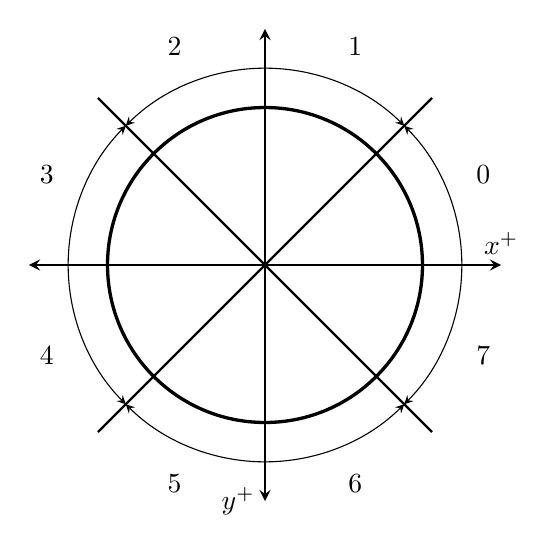
\begin{tikzpicture}[>=stealth]
	\draw [very thick] (0,0) circle (2);

	%% Coordinate axes
	\draw [<->,thick] (-3,0) -- (3,0) node [above] {$x^+$};
	\draw [<->,thick] (0,3) -- (0,-3) node [left] {$y^+$};

	%% Diagonals
	\draw [thick] (0,0) +(45:-3) -- (45:3);
	\draw [thick] (0,0) +(135:-3) -- (135:3);

	%% Even arcs
	\foreach \x in {0,1,2,3} {
		\pgfmathmultiply{\x}{90}
		\pgfmathtruncatemacro{\alpha}{\pgfmathresult}
		\draw [->] (0,0) +(0+\alpha:2.5cm) arc (0+\alpha:45+\alpha:2.5cm);
		\pgfmathmultiply{\x}{2}
		\pgfmathtruncatemacro{\arclabel}{\pgfmathresult}
		\path (0,0) +(22.5+\alpha:3cm) node {$\arclabel$};
	}

	%% Odd arcs
	\foreach \x in {0,1,2,3} {
		\pgfmathmultiply{\x}{90}
		\pgfmathtruncatemacro{\alpha}{\pgfmathresult}
		\draw [->] (0,0) +(90+\alpha:2.5cm) arc (90+\alpha:90+\alpha-45:2.5cm);
		\pgfmathparse{2*\x+1}
		\pgfmathtruncatemacro{\arclabel}{\pgfmathresult}
		\path (0,0) +(67.5+\alpha:3cm) node {$\arclabel$};
	}
\end{tikzpicture}

			\caption{Octants in the Eight-Way Symmetry of a Circle}
			\label{fig:eightsymmetry}
		\end{figure}
		Because it is necessary that the points are ordered
		counterclockwise from the positive x-axis, we modify the
		algorithm. The algorithm calculates the points from ordered
		clockwise or counterclockwise from the closest coordinate axis.
		Hence, we reverse the points calculated for every odd octant and
		then concatenate their data points.

		\begin{algorithm}[ht!]
			\caption{Ordered Bresenham Circle Algorithm}
			\begin{algorithmic}
				\Ensure{points returned are ordered counterclockwise from the positive x-axis}
				\Procedure{BresenhamCircle}{origin, radius}
					\State $x \gets$ radius
					\State $y \gets 0$
					\State $r_{\text{error}} \gets 1 - x$
					\State octants $\gets$ empty array
					\While{$x \geq y$}
						\State octants[0] $\Leftarrow$ ($x$ + origin.x, $-y$ + origin.y)
						\State octants[1] $\Leftarrow$ ($y$ + origin.x, $-x$ + origin.y)
						\State octants[2] $\Leftarrow$ ($-y$ + origin.x, $-x$ + origin.y)
						\State octants[3] $\Leftarrow$ ($-x$ + origin.x, $-y$ + origin.y)
						\State octants[4] $\Leftarrow$ ($-x$ + origin.x, $y$ + origin.y)
						\State octants[5] $\Leftarrow$ ($-y$ + origin.x, $x$ + origin.y)
						\State octants[6] $\Leftarrow$ ($y$ + origin.x, $x$ origin.y)
						\State octants[7] $\Leftarrow$ ($x$ + origin.x, $y$ origin.y)
						\State $y \gets y + 1$
						\If{$r_{\text{error}} < 0$}
							\State $r_{\text{error}} \gets r_{\text{error}} + 2y + 1$
						\Else
							\State $x \gets x - 1$
							\State $r_{\text{error}} \gets r_{\text{error}} + 2(y - x + 1)$
						\EndIf
					\EndWhile
					\State points $\gets$ []
					\ForAll{octant $\in$ octants}
						\If{octant is odd}
							\State reverse the octant
						\EndIf
						\ForAll{point $\in$ octant}
							\State points $\Leftarrow$ point
						\EndFor
					\EndFor
					\State \Return points
				\EndProcedure
			\end{algorithmic}
		\end{algorithm}

	% subsubsection Ordered Bresenham Circle Algorithm (end)
% section Pseudo Code (end)

\end{document}
